% Source: bigram_multinomial_logistic_regression.tex
\begin{notechapter}
\chapter{Bigram Language Modeling with Multinomial Logistic Regression}\label{ch:bigram-logreg-model}

\section{Introduction}
This document explains the multinomial logistic regression model applied to
bigram language modeling. The goal is to estimate the probability
\( P(\text{word}_2 \mid \text{word}_1) \), where \(\text{word}_1\) is the
previous word and \(\text{word}_2\) is the next word. The model uses a
single-layer neural network with a softmax activation function.

\section{Model Diagram with Bias Term}
The following diagram illustrates the structure of the model, including the
bias term:

\begin{center}
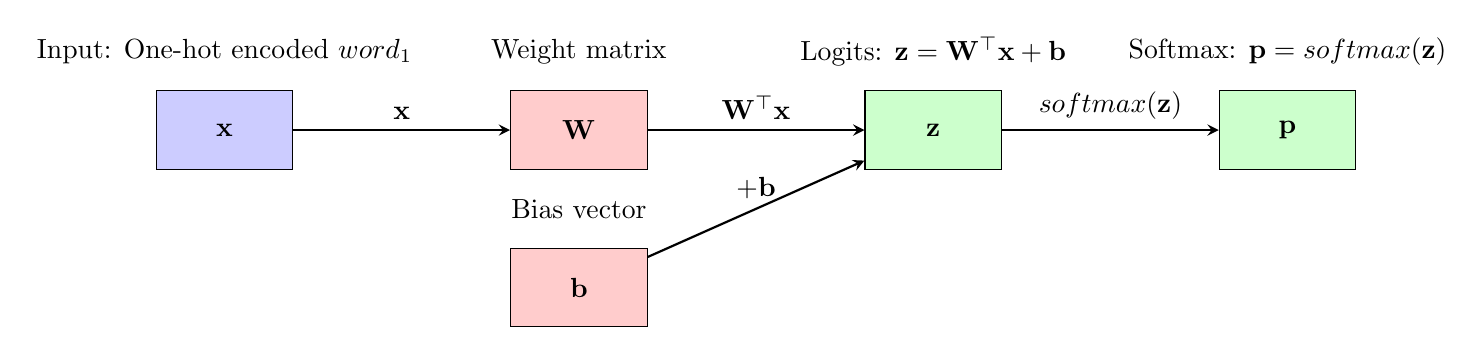
\begin{tikzpicture}[
    node distance=1.5cm,
    input/.style={rectangle, draw, fill=blue!20, text width=1.5cm, text centered, minimum height=1cm},
    output/.style={rectangle, draw, fill=green!20, text width=1.5cm, text centered, minimum height=1cm},
    param/.style={rectangle, draw, fill=red!20, text width=1.5cm, text centered, minimum height=1cm},
    arrow/.style={thick,->,>=stealth}
]
    % Input layer
    \node[input] (x) {$\mathbf{x}$};
    \node[above of=x, yshift=-0.5cm] (input_label) {Input: One-hot encoded $\text{word}_1$};

    % Weight matrix
    \node[param, right of=x, xshift=3cm] (W) {$\mathbf{W}$};
    \node[above of=W, yshift=-0.5cm] (W_label) {Weight matrix};

    % Bias vector
    \node[param, below of=W, yshift=-0.5cm] (b) {$\mathbf{b}$};
    \node[above of=b, yshift=-0.5cm] (b_label) {Bias vector};

    % Logits
    \node[output, right of=W, xshift=3cm] (z) {$\mathbf{z}$};
    \node[above of=z, yshift=-0.5cm] (z_label) {Logits: $\mathbf{z} = \mathbf{W}^\top \mathbf{x} + \mathbf{b}$};

    % Softmax
    \node[output, right of=z, xshift=3cm] (p) {$\mathbf{p}$};
    \node[above of=p, yshift=-0.5cm] (p_label) {Softmax: $\mathbf{p} = \text{softmax}(\mathbf{z})$};

    % Arrows
    \draw[arrow] (x) -- (W) node[midway, above] {$\mathbf{x}$};
    \draw[arrow] (W) -- (z) node[midway, above] {$\mathbf{W}^\top \mathbf{x}$};
    \draw[arrow] (b) -- (z) node[midway, above] {$+ \mathbf{b}$};
    \draw[arrow] (z) -- (p) node[midway, above] {$\text{softmax}(\mathbf{z})$};

\end{tikzpicture}
\end{center}

\subsection{Explanation of the Diagram}
\begin{itemize}
    \item The input \(\mathbf{x}\) is a one-hot encoded vector representing
          \(\text{word}_1\).
    \item The weight matrix \(\mathbf{W}\) maps the input to the logits
          \(\mathbf{z}\).
    \item The bias term \(\mathbf{b}\) adds flexibility to the model by
          allowing it to learn an offset for each output class.
    \item The softmax function converts the logits \(\mathbf{z}\) into
          probabilities \(\mathbf{p}\).
\end{itemize}

\section{Model Diagram without Bias Term}
The following diagram illustrates the structure of the model without the bias
term:


\begin{minipage}[t]{.62\textwidth}
\raggedright
\begin{center}
      \tikzset{%
        every neuron/.style={
          circle,
          draw,
          minimum size=1cm
        },
        neuron missing/.style={
          draw=none, 
          scale=4,
          text height=0.333cm,
          execute at begin node=\color{black}$\vdots$
        },
      }

      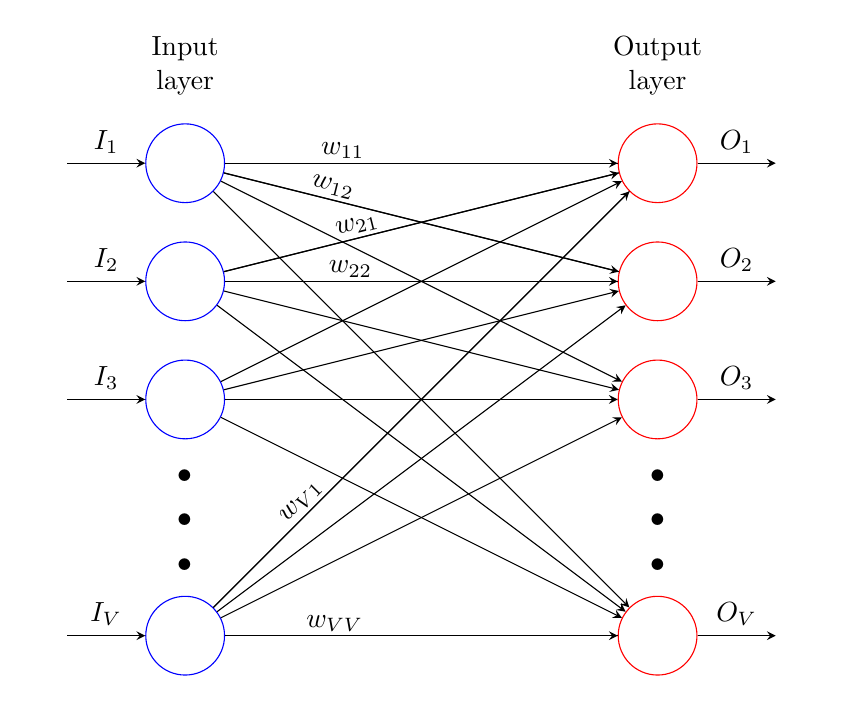
\begin{tikzpicture}[x=1.5cm, y=1.5cm, >=stealth]
      
      \foreach \m/\l [count=\y] in {1,2,3,missing,4}
        \node [every neuron/.try, neuron \m/.try, color=blue] (input-\m) at (0,2.5-\y) {};
      
      \foreach \m [count=\y] in {1,2,3,missing,4}
        \node [every neuron/.try, neuron \m/.try, color=red] (output-\m) at (4,2.5-\y) {};
      
      \foreach \l [count=\i] in {1,2,3,V}
        \draw [<-] (input-\i) -- ++(-1,0)
          node [above, midway] {$I_\l$};
      
      \foreach \l [count=\i] in {1,2,3,V}
        \draw [->] (output-\i) -- ++(1,0)
          node [above, midway] {$O_\l$};
      
      % Label weights only for i=1 and i=V
      \foreach \j in {1,...,4} {
        \draw [->] (input-1) -- (output-\j);
        \draw [->] (input-4) -- (output-\j);
      }
      
      \draw (input-1) -- (output-1)
          node [midway, above, sloped, xshift={-1.0cm}, yshift={-0.07cm}] {$w_{11}$};
      \draw (input-1) -- (output-2)
          node [midway, above, sloped, xshift={-1.2cm}, yshift={-0.07cm}] {$w_{12}$};
          
      \draw (input-2) -- (output-1)
          node [midway, above, sloped, xshift={-0.8cm}, yshift={-0.07cm}] {$w_{21}$};
      
      \draw (input-2) -- (output-2)
          node [midway, above, sloped, xshift={-0.9cm}, yshift={-0.07cm}] {$w_{22}$};
      
      \draw (input-4) -- (output-1)
          node [midway, above, sloped, xshift={-2.0cm}, yshift={-0.07cm}] {$w_{V1}$};
      \draw (input-4) -- (output-4)
          node [midway, above, sloped, xshift={-1.1cm}, yshift={-0.07cm}] {$w_{VV}$};
      
      % Draw connections for i=2 and i=3 without labels
      \foreach \i in {2,3}
        \foreach \j in {1,...,4}
          \draw [->] (input-\i) -- (output-\j);
      
      \foreach \l [count=\x from 0] in {Input, Output}
        \node [align=center, above] at (\x*4,2) {\l \\ layer};
      
      \end{tikzpicture}
      \end{center}
\end{minipage}
\hfill
\noindent
\begin{minipage}[t]{.34\textwidth}
\raggedleft
\[
\mathbf{x} = 
\begin{bmatrix}
I_{1} \\
I_{2} \\
\vdots \\
I_{V}
\end{bmatrix}
\]

\[
\mathbf{W} = 
\begin{bmatrix}
w_{11} & w_{12} & \cdots & w_{1V} \\
w_{21} & w_{22} & \cdots & w_{2V} \\
\vdots & \vdots & \ddots & \vdots \\
w_{V1} & w_{V2} & \cdots & w_{VV}
\end{bmatrix}
\] 

\[
\mathbf{W}^\top \mathbf{x} = 
\begin{bmatrix}
w_{11} I_1 + w_{21} I_2 + \cdots + w_{V1} I_V \\
w_{12} I_1 + w_{22} I_2 + \cdots + w_{V2} I_V \\
\vdots \\
w_{1V} I_1 + w_{2V} I_2 + \cdots + w_{VV} I_V
\end{bmatrix}
\]
\end{minipage}

\subsection{Explanation of the Diagram}
\begin{itemize}
    \item The input layer consists of \( V \) neurons, where \( V \) is the
          vocabulary size. Each neuron corresponds to a one-hot encoded input
          \( I_1, I_2, \dots, I_V \). For example, if \(\text{word}_1\) is the
          \(i\)-th word in the vocabulary, then \( I_i = 1 \) and all other
          \( I_j = 0 \).\\
          Therefore, $\mathbf{W}^\top \mathbf{x}$ is equal to the transpose
          of the $i^{\text{th}}$ line of the matrix $\mathbf{W}$.\\
          For example,
          \[
            \mathbf{W}^{T} \mathbf{x} = 
            \begin{bmatrix}
            w_{11} & w_{21} & \cdots & w_{V1} \\
            w_{12} & w_{22} & \cdots & w_{V2} \\
            \vdots & \vdots & \ddots & \vdots \\
            w_{1V} & w_{2V} & \cdots & w_{VV}
            \end{bmatrix}
            \begin{bmatrix}
                  1 \\
                  0 \\
                  \vdots \\
                  0
            \end{bmatrix} =
            \begin{bmatrix}
                  w_{11} \\ w_{12} \\ \vdots \\ w_{1V}
            \end{bmatrix}
            \]
    \item The output layer also consists of \( V \) neurons, representing the
          output probabilities \( O_1, O_2, \dots, O_V \). These probabilities
          are computed using the softmax function:
          \[
          O_j = P(\text{word}_2 = j \mid \text{word}_1) =
          \text{softmax}(\mathbf{z})_j = \frac{e^{z_j}}{\sum_{k=1}^V e^{z_k}}.
          \]
    \item The connections between the input and output layers represent the
          weight matrix \(\mathbf{W}\), which maps the input to the logits
          \(\mathbf{z}\).
\end{itemize}

\section{Problem Setup}
The goal is to estimate the probability \( P(\text{word}_2 \mid \text{word}_1) \),
where \(\text{word}_1\) is the previous word and \(\text{word}_2\) is the next
word. The input is a one-hot encoded vector representing \(\text{word}_1\), and
the output is a probability distribution over the vocabulary for \(\text{word}_2\).

\section{Notation}
\begin{itemize}
    \item Let the vocabulary size be \( V \).
    \item Let \(\mathbf{x} \in \mathbb{R}^V\) be the one-hot encoded input
          vector for \(\text{word}_1\). For example, if \(\text{word}_1\) is
          the \(i\)-th word in the vocabulary, then:
          \[
          \mathbf{x} = [0, 0, \dots, 1, \dots, 0]^\top,
          \]
          where the \(i\)-th element is 1 and all others are 0.
    \item Let \(\mathbf{W} \in \mathbb{R}^{V \times V}\) be the weight matrix,
          where each row corresponds to the weights for predicting a specific
          word in the vocabulary.
    \item Let \(\mathbf{z} \in \mathbb{R}^V\) be the logits (unnormalized
          scores) for each word in the vocabulary.
\end{itemize}

\section{Forward Pass}
\begin{itemize}
    \item Compute the logits \(\mathbf{z}\):
          \[
          \mathbf{z} = \mathbf{W}^\top \mathbf{x}.
          \]
          Since \(\mathbf{x}\) is one-hot encoded, this simplifies to selecting
          the \(i\)-th row of \(\mathbf{W}\) (where \(\mathbf{x}_i = 1\)):
          \[
          \mathbf{z} = \mathbf{W}_i,
          \]
          where \(\mathbf{W}_i\) is the \(i\)-th row of \(\mathbf{W}\).

    \item Apply the softmax function to convert logits \(\mathbf{z}\) into
          probabilities:
          \[
          P(\text{word}_2 = j \mid \text{word}_1 = i) =
          \text{softmax}(\mathbf{z})_j = \frac{e^{z_j}}{\sum_{k=1}^V e^{z_k}}.
          \]
          Here, \(j\) indexes the vocabulary, and
          \(\text{softmax}(\mathbf{z})_j\) is the probability of \(\text{word}_2\)
          being the \(j\)-th word in the vocabulary.
\end{itemize}

\section{Training}
The model is trained using \textbf{cross-entropy loss}. For a single training
example \((\text{word}_1, \text{word}_2)\), the loss is:
\[
\mathcal{L} = -\log P(\text{word}_2 \mid \text{word}_1).
\]
If \(\text{word}_2\) is the \(j\)-th word in the vocabulary, then:
\[
\mathcal{L} = -\log \left( \text{softmax}(\mathbf{z})_j \right).
\]
The gradients of the loss with respect to the parameters (\(\mathbf{W}\)) are
computed using backpropagation, and the parameters are updated using gradient
descent.

\section{Gradient Computation}
\subsection{Gradient of the Loss with Respect to the Logits}
The gradient of the cross-entropy loss with respect to the logits \(\mathbf{z}\)
is:
\[
\frac{\partial \mathcal{L}}{\partial z_j} =
P(\text{word}_2 = j \mid \text{word}_1) - \mathbb{I}(\text{word}_2 = j),
\]
where:
\begin{itemize}
    \item \(P(\text{word}_2 = j \mid \text{word}_1)\) is the predicted
          probability for the \(j\)-th word.
    \item \(\mathbb{I}(\text{word}_2 = j)\) is an indicator function that is 1
          if \(\text{word}_2\) is the \(j\)-th word and 0 otherwise.
\end{itemize}

\subsection{Gradient with Respect to the Parameters}
The logit \(z_j\) is computed as:
\[
z_j = \mathbf{W}_j^\top \mathbf{x}.
\]
Therefore, the gradient of the loss with respect to \(\mathbf{W}_j\) is:
\[
\frac{\partial \mathcal{L}}{\partial \mathbf{W}_j} =
\frac{\partial \mathcal{L}}{\partial z_j} \cdot \mathbf{x}.
\]
Since \(\mathbf{x}\) is one-hot encoded, this simplifies to:
\[
\frac{\partial \mathcal{L}}{\partial \mathbf{W}_j} =
\left( P(\text{word}_2 = j \mid \text{word}_1) -
\mathbb{I}(\text{word}_2 = j) \right) \cdot \mathbf{x}.
\]

\section{Gradient Descent Update}
Update the parameters using gradient descent:
\[
\mathbf{W}_j \leftarrow \mathbf{W}_j - \eta \frac{\partial \mathcal{L}}{\partial \mathbf{W}_j},
\]
where \(\eta\) is the learning rate.

\section{Example}
Suppose:
\begin{itemize}
    \item Vocabulary: \(\{ \text{cat}, \text{dog}, \text{mouse} \}\) (size \(V = 3\)).
    \item \(\text{word}_1 = \text{cat}\) (one-hot encoded as \([1, 0, 0]^\top\)).
    \item \(\text{word}_2 = \text{dog}\) (index \(j = 2\)).
\end{itemize}

\begin{itemize}
    \item Compute the predicted probabilities using softmax.
    \item Compute the gradients:
          \[
          \frac{\partial \mathcal{L}}{\partial \mathbf{W}_2} =
          \left( P(\text{word}_2 = \text{dog} \mid \text{word}_1 = \text{cat}) - 1 \right)
          \cdot [1, 0, 0]^\top.
          \]
    \item Update \(\mathbf{W}_2\) using gradient descent.
\end{itemize}

\section{Why the Bias Term is Sometimes Dropped}
In some cases, the bias term \(\mathbf{b}\) is omitted from the model. This is
common in models like Word2Vec, where the focus is on learning high-quality
word embeddings rather than precise probabilities. Here are some reasons why
the bias term might be dropped:

\begin{itemize}
    \item \textbf{Simplified Objective:} In models like Word2Vec, the goal is to
          learn distributed representations (embeddings) of words. The dot
          product between embeddings is sufficient to capture the relationship
          between words, and the bias term is not necessary.
    \item \textbf{Efficiency:} Omitting the bias term reduces the number of
          parameters, making the model simpler and faster to train.
    \item \textbf{Normalization:} The softmax function normalizes the logits into
          probabilities, and the bias term is not required for this
          normalization.
\end{itemize}

However, in most cases, including the bias term is recommended because it adds
flexibility to the model and improves its ability to fit the data.
\end{notechapter}
